\begin{exercice*}
    Pour chaque figure, indiquer les caractéristiques de la rotation de centre $C$ qui transforme $A$ en $B$. C'est à dire son angle et son sens.
    \begin{enumerate}
        \item $ABC$ est un triangle rectangle et isocèle en $C$.
        \begin{tikzpicture}[scale=0.7]
            \coordinate[label=above:$A$] (A) at (1,4);
            \coordinate[label=right:$B$] (B) at (4,1);
            \coordinate[label=below left:$C$] (C) at (1,1);
            \draw (A)--(B)--(C)--cycle;
            \tkzMarkRightAngles[size=0.3](B,C,A);
            \tkzMarkSegments[color=red,pos=0.5, mark=oo](A,C C,B);
        \end{tikzpicture}
        \item $ABC$ est un triangle équilatéral.\\
        \begin{tikzpicture}[scale=0.7]
            \coordinate[label=below:$A$] (A) at (1,1);
            \coordinate[label=above:$B$] (B) at (3,4);
            \tkzDefPointBy[rotation=center A angle -60](B);
            \tkzGetPoint{C};
            \tkzLabelPoint[below](C){$C$};
            \draw (A)--(B)--(C)--cycle;        
            \tkzMarkSegments[color=red,pos=0.5, mark=oo](A,C C,B B,A);
        \end{tikzpicture}
        \item $ABC$ est un triangle isocèle de sommet principal $C$ tel que l'angle à la base vaut \ang{55}.\\
        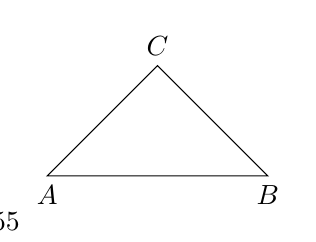
\begin{tikzpicture}[scale=0.7]
            \coordinate[label=below:$A$] (A) at (1,1);
            \coordinate[label=below:$B$] (B) at (5,1);
            \coordinate[label=above:$C$] (C) at (3,3);
            \draw (A)--(B)--(C)--cycle;        
            \tkzMarkSegments[color=red,pos=0.5, mark=oo](A,C C,B);
            \tkzMarkAngle[size=0.6](B,A,C);
            \tkzLabelAngle[pos=1](B,A,C){$\ang{55}$};
        \end{tikzpicture}
    \end{enumerate}
\end{exercice*}
\begin{corrige}
    %\setcounter{partie}{0} % Pour s'assurer que le compteur de \partie est à zéro dans les corrigés
    % \phantom{rrr}    
    Pour chaque figure, indiquer les caractéristiques de la rotation de centre $C$ qui transforme $A$ en $B$. C'est à dire son angle et son sens.

    \begin{enumerate}
        \item $ABC$ est un triangle rectangle et isocèle en $C$.        
        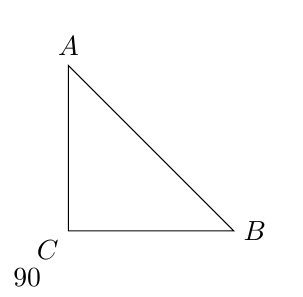
\begin{tikzpicture}[scale=0.7]
            \coordinate[label=above:$A$] (A) at (1,4);
            \coordinate[label=right:$B$] (B) at (4,1);
            \coordinate[label=below left:$C$] (C) at (1,1);
            \draw (A)--(B)--(C)--cycle;
            \tkzMarkRightAngles[size=0.3](B,C,A);
            \tkzMarkSegments[color=red,pos=0.5, mark=oo](A,C C,B);
            \tkzPicAngle["{\red $\ang{90}$}",draw=red,<-,angle eccentricity=1.4,angle radius=0.7cm](B,C,A);
        \end{tikzpicture}

        {\red Rotation d'angle \ang{90} dans le sens des aiguilles d'une montre, sens horaire ou sens négatif.}
        \item $ABC$ est un triangle équilatéral.\\
        \begin{tikzpicture}[scale=0.7]
            \coordinate[label=below:$A$] (A) at (1,1);
            \coordinate[label=above:$B$] (B) at (3,4);
            \tkzDefPointBy[rotation=center A angle -60](B);
            \tkzGetPoint{C};
            \tkzLabelPoint[below](C){$C$};
            \draw (A)--(B)--(C)--cycle;        
            \tkzMarkSegments[color=red,pos=0.5, mark=oo](A,C C,B B,A);
            \tkzPicAngle["{\red $\ang{60}$}",draw=red,<-,angle eccentricity=1.4,angle radius=0.7cm](B,C,A);
        \end{tikzpicture}

        {\red Rotation d'angle \ang{60} dans le sens des aiguilles d'une montre, sens horaire ou sens négatif.}
        \item $ABC$ est un triangle isocèle de sommet principal $C$ tel que l'angle à la base vaut \ang{55}.\\
        \begin{tikzpicture}[scale=0.7]
            \coordinate[label=below:$A$] (A) at (1,1);
            \coordinate[label=below:$B$] (B) at (5,1);
            \coordinate[label=above:$C$] (C) at (3,3);
            \draw (A)--(B)--(C)--cycle;        
            \tkzMarkSegments[color=red,pos=0.5, mark=oo](A,C C,B);
            \tkzMarkAngle[size=0.6](B,A,C);
            \tkzLabelAngle[pos=1](B,A,C){$\ang{55}$};
            \tkzPicAngle["{\red $\ang{70}$}",draw=red,->,angle eccentricity=1.4,angle radius=0.7cm](A,C,B);
        \end{tikzpicture}

        {\red La somme des angles d'un triangle vaut \ang{180}, et les angles à la base d'un triangle isocèle sont égaux donc $\widehat{ACB}=\ang{180}-2\times \ang{55}=\ang{70}$.
        
        D'où rotation d'angle \ang{70} dans le sens inverse des aiguilles d'une montre, sens anti-horaire ou sens positif.}
    \end{enumerate}
\end{corrige}

